% PREAMBLE Version 0.1

% DO NOT COMPILE THIS FILE ALONE

% Document classes
% ----------------
\documentclass[a4paper, 11pt, oneside]{article}
% \documentclass[a4paper,landscape]{article}

% Project structure
% -----------------
\usepackage{subfiles}

% Spacing, margins, etc.
% ----------------------
\usepackage{geometry}
\usepackage{float}
\usepackage{fullpage}
\usepackage{indentfirst}
\usepackage[francais]{babel}
% \usepackage[english]{babel}

% Encoding, characters, fonts, etc.
% ---------------------------------
\usepackage[T1]{fontenc}
\usepackage[utf8]{inputenc}
% \usepackage{upgreek}
\usepackage{eurosym}
\usepackage{amsfonts}
\usepackage{amssymb}
\usepackage{textcomp}

% Figures
% -------
\usepackage{graphicx}
% \usepackage{subfigure}

% Colors
% ------
% \usepackage{color}
\usepackage[table]{xcolor}

% URLs and refs
% -------------
% \usepackage{url}
% \usepackage{hyperref}
% \usepackage[bottom]{footmisc}
% \usepackage[all]{hypcap}

% Environments
% ------------
\usepackage{amsmath}
\usepackage{amsthm}
\usepackage{array}
\usepackage{tabularx}
\usepackage{enumerate}
\usepackage{enumitem}
\usepackage{listings}
\usepackage{framed}
\usepackage[framed]{matlab-prettifier}
\usepackage{booktabs}
\usepackage{algorithm}
\usepackage{algorithmic}

% =================================================================================
%                                   New commands
% =================================================================================



\renewcommand{\thesubsection}{\alph{subsection})}
\renewcommand{\thesubsubsection}{\roman{subsubsection})}
\usepackage{clrscode3e}

\begin{document}

\subfile{titlepage.tex}

\section{Analyse théorique}
\subsection{} %a
	Pour implémenter la structure Union-Find à l'aide d'un arbre binaire, nous avons décidé de créer un vecteur dont chaque élément est initialement la racine d'un arbre binaire. Chaque arbre du vecteur représente donc un singleton. Lorsque nous procédons a une union, nous utilisons l'implémentation des arbres binaires vue au cours théorique.
	\begin{figure}[h]
		\caption{Après UfCreate}
		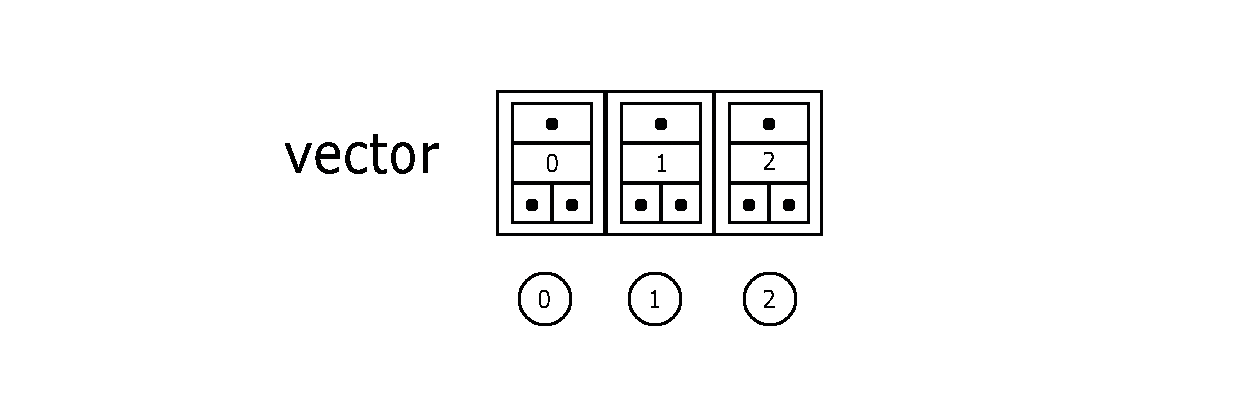
\includegraphics[scale=0.75]{1}
	\end{figure}

	\begin{figure}[h]
		\caption{Après UfUnion}
		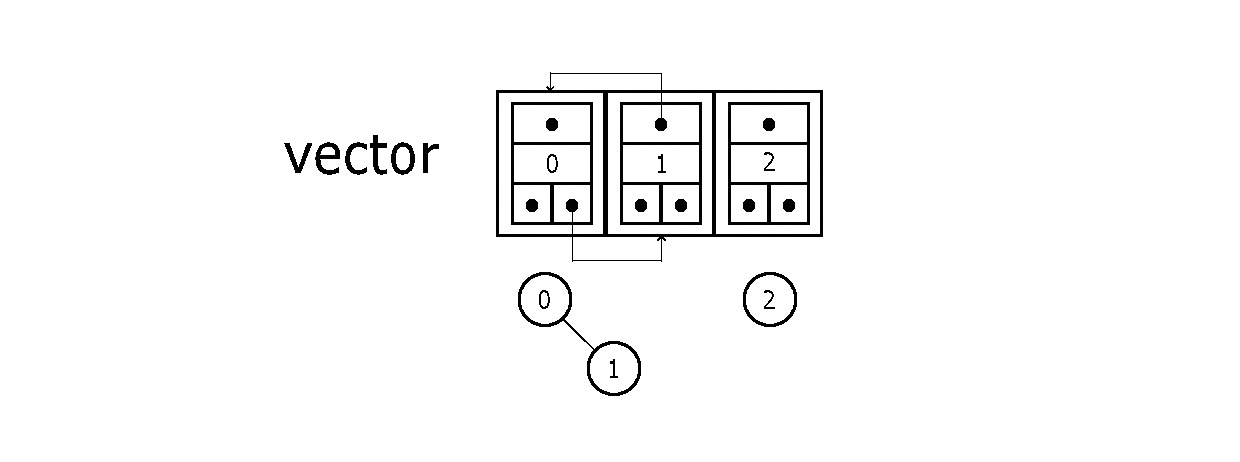
\includegraphics[scale=0.75]{2}
	\end{figure}

\subsection{} %b
La complexité de \textit{ufFind} dans l'implémentation par listes est dans le meilleur cas $\Theta(Q)$ et dans le pire cas $\Theta(Q^2)$.

La complexité de \textit{ufUnion} dans l'implémentation par listes est identique à la complexité de \textit{ufFind} puisqu'elle utilise cette fonction. Nous avons donc $\Theta(Q)$ dans le meilleur cas et $\Theta(Q^2)$ dans le pire cas.

	\begin{tabular}{|l||c|c|}
	\hline
  & Liste & Arbre\\
  \hline\hline
  Fonction UfUnion & & O(h)\footnote{h étant le nombre d'étage qu'il faut monter pour arriver à la racine} \\
  Fonction UfFind & & \\
  \hline
\end{tabular}

\subsection{} %c
\subsection{} %d

\subsection{La structure de labyrinthe} %c
La structure maze est composée de 4 éléments.
\begin{itemize}
\item size : contient la taille du labyrinthe. Pour une taille N, le labyrinthe sera un carré N x N.
\item unionFind : contient l'ensemble disjoint qui a été utilisé pour créer le labyrinthe.
\item neighbours : est un vecteur contenant les paires de cellules étant voisines et un booléen égal à \textit{true} si elles sont séparées par un mur, à \textit{false} sinon.
\item convert : est une matrice permettant de retrouver le numéro d'une case du labyrinthe à partir de ses coordonnées.
\bigbreak
En effet, nous avons choisi d'utiliser la plupart du temps des entiers pour identifier les cases afin de pouvoir utiliser la structure \textit{UnionFind} préalablement définie (et qui contenait des entiers). Ainsi nous représentons chaque case par un chiffre de $0$ à $N *N - 1$
\end{itemize}

\subsection{Pseudocode} %d
\begin{codebox}
\Procname{$\proc{mzCreate}(size)$}
\li $\proc{Maze } maze$
\li $maze.size = size$
\li $maze.neighbours =$ all pairs of cells that are neighbours with a wall between each of them
\li $maze.unionFind = \proc{ufCreate}(size)$
\li \While $\proc{ufComponentsCount}(maze.unionFind) > 1$
\Do
\li 	$(coord1, coord2) =$ a random pair of neighbours
\li		\If There is a wall
\li \Then $\proc{mzSetWall}(maze, coord1, coord2, false)$ //Remove the wall
\li	$\proc{ufUnion}(maze.unionFind, coord1, coord2)$
\End
\End
\li \Return $maze$
\End
\end{codebox}

\begin{codebox}
\Procname{$\proc{mzIsValid}(maze)$}
\li \If $\proc{ufComponentsCount}(maze.unionFind) > 1$
\li \Then \Return $false$
\li \Else
\li \Return $true$
\End
\End
\end{codebox}

\subsection{Complexité en temps avec UnionFindList} %e
La complexité de \proc{mzCreate} est dans le meilleur cas est de $\Theta(Q^2)$ puisqu'il faut au minimum $Q-1$ unions pour rassembler tous les sous-ensembles et que la complexité au meilleur cas de \textit{ufUnion} est de $\Theta(Q)$.

La complexité au pire cas est difficile à définir puisque l'on choisi un mur à retirer de manière aléatoire parmi tous les "emplacements possibles" de murs. Il faut donc tomber si un emplacement contenant un mur pour avancer dans la fonction.

\bigbreak
\proc{mzIsValid} est constant puisqu'il s'agit simplement d'aller lire la taille de l'\textit{UnionFind}.

\section{Analyse empirique}
\subsection{} %a
	\begin{figure}[h]
		\caption{Implémentation par liste}
		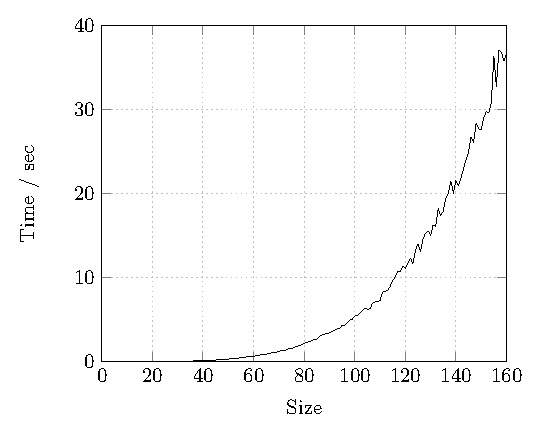
\includegraphics{Tests/List/list}
	\end{figure}

	\begin{figure}[h]
		\caption{Implémentation par Arbre}
		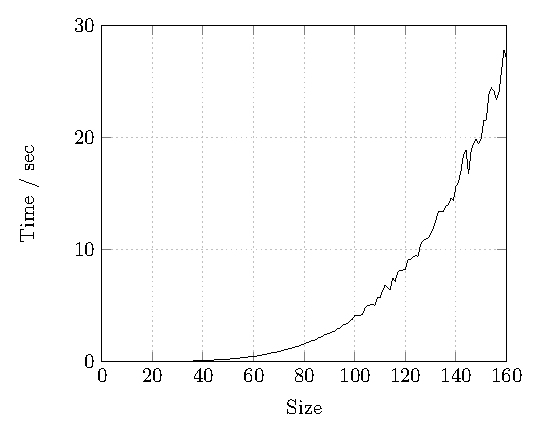
\includegraphics{Tests/Tree/tree}
	\end{figure}

\subsection{} %b

\end{document}
